\documentclass[
11pt, paper=a4,  listof=totocnumbered, % lists are also included in table of contents
numbers=noendperiod, % Don't add a period at the end of a chapter number
]{scrreprt}

    \usepackage{chngcntr}
    \counterwithout{footnote}{chapter}
    \counterwithout{figure}{chapter}
        \counterwithout{table}{chapter}
    
% ===============================
% IUBH Template für Seminar-, Bachelor-, and Master-works
% -------------------------------
% Authors; Ralf Kneuper, Jörg Sawatzki
% Maintainer: Paul Libbrecht

% Fix of Warning: Class scrreprt Warning: \float@addtolists detected!
% https://komascript.de/faq_float%40addtolist
\usepackage{scrhack}

\usepackage{mathtools}
% get custom bibliography style working without prepending [brackets]
\usepackage{natbib}
\setcitestyle{aysep={}} % remove comma as delimiter 

% breaks line at hyphens (resolves formatting issues in bibliography)
\usepackage[hyphens]{url}

\usepackage{txfonts} % Use a Times-new-roman open-source clone

% if you insist on Arial... then uncomment the following
\usepackage{helvet}
\renewcommand{\familydefault}{\sfdefault}

\usepackage{caption}
\usepackage{float}

\setkomafont{chapter}{\Large} 
\setkomafont{section}{\large}
\setkomafont{subsection}{\large} 

\usepackage[left=2cm,right=2cm,top=2cm,bottom=2cm]{geometry} % margins
\addtolength{\footskip}{-0.7cm}% foot larger by 0,7 cm  (Raises the page number)


\usepackage[onehalfspacing]{setspace} % line space 1,5

\setlength{\parindent}{6pt} % Indent at start of paragraphs  6pt

\usepackage[utf8]{inputenc} %UTF-8 to encode many characters => for many characters, you can just input the character and avoid a macro

\usepackage[english]{babel} % english hyphenations
%\usepackage[T1]{fontenc} %wichtig für Trennung von Wörtern mit Umlauten
\usepackage{microtype} % align margins

\usepackage{graphicx} % import graphics
\usepackage{placeins}% places the graphics within text

% Abbreviation's directory
% printonlyused - only if used
% withpage - the first occurrence's page number is listed too
\usepackage[withpage]{acronym}

\usepackage[hidelinks]{hyperref} %https://tex.stackexchange.com/questions/823/remove-ugly-borders-around-clickable-cross-references-and-hyperlinks

\usepackage{listings}
\usepackage{color}

\definecolor{dkgreen}{rgb}{0,0.6,0}
\definecolor{gray}{rgb}{0.5,0.5,0.5}
\definecolor{mauve}{rgb}{0.58,0,0.82}

\lstset{frame=tb,
  language=python,
  aboveskip=3mm,
  belowskip=3mm,
  showstringspaces=false,
  columns=flexible,
  stepnumber=1,
  numberfirstline=true,
  numbers=left,
  basicstyle={\small\ttfamily},
  numberstyle=\tiny\color{gray},
  keywordstyle=\color{blue},
  commentstyle=\color{dkgreen},
  stringstyle=\color{mauve},
  breaklines=true,
  breakatwhitespace=true,
  tabsize=2
}

\begin{document}

%TITELBLATT:!!!!!!!!!!!!!!!!!!!!!!!!!!!!!!!!!!!!!!!!!!!!!!!!!!!!!!!!!!!!!!!!!!!!!!!!!!!!!!!!!!!!!!!!!!!!!

\label{titlePage}
\begin{figure}[h]
\centering
\advance\leftskip--2cm

\includegraphics[width=0.50\textwidth]{pics/logo.pdf}
\end{figure}
\FloatBarrier

\begin{Large} 
\begin{center}
Workbook
\end{center}
\end{Large} 

\vspace*{5mm}

\begin{large} 
\begin{center}
University of Applied Science - Online
\end{center}
\end{large} 

\begin{large} 
\begin{center}
Study-branch: PLEASE ADAPT ALL ASPECTS TO MATCH REQUIREMENTS
\end{center}
\end{large}

\vspace*{15mm}

\begin{Large} 
\begin{center}
\textbf{<THIS IS THE TITLE TO BE ADAPTED>}
\end{center}
\end{Large}

\vspace*{15mm}

\begin{large} 
\begin{center}
Prannoy Mulmi
\end{center}
\end{large} 

\vspace*{-6mm}

\begin{large} 
\begin{center}
Matrikelnummer: 010101001
\end{center}
\end{large} 

\vspace*{-6mm}

\begin{large} 
\begin{center}
Straße 10
\end{center}
\end{large} 

\vspace*{-6mm}

\begin{large} 
\begin{center}
realized in....
\end{center}
\end{large} 

\vspace*{5mm}

\begin{large} 
\begin{center}
Advisor: <Advisor>
\end{center}
\end{large} 

\begin{large} 
\begin{center}
Realized with input of the Parameter Generator: <Signature-Hash> $\Omega \longrightarrow R^2$
\end{center}
\end{large} 



\vspace*{-6mm}

\begin{large} 
\begin{center}
Delivery date: 1.1.1970
\end{center}
\end{large} 


\pagestyle{empty} % no page numbering on the cover



\renewcommand{\thechapter}{\Roman{chapter}}

\pagestyle{plain}

\pagenumbering{Roman} %the intro is counted with roman numbers
\setcounter{page}{2} %starting with page 2 (page 1 is the titel)

% --- too detailed for a seminar but otherwise useful
%\chapter{Blocking notice (optional)}

Useful if this document contains information that should prevent redistribution.
%\chapter{Acknoowledgements (optional)}

Thanks to....
%\chapter{Abstract}



\tableofcontents %table of contents
\listoffigures %List of figures
%\listoftables %list of tables

% Abbreviations list
\renewcommand\refname{Abbreviations} \chapter{Abbreviations}
% The abbreviations list should contain all abbreviations that are not common-knowledge.
\begin{acronym}[NMWC] % the longest abbreviation here (for layout)
    \setlength {\itemsep}{-\parsep} % geringerer Zeilenabstand    	 

    \acro{CDF}{Cumulative Distribution Function}
    \acro{CCDF}{Complementary Cumulative Distribution Function}
    \acro{DOF}{Degrees Of Freedom}
    \acro{PDF}{Probability Density Function}
    \acro{PMF}{Probability Mass Function}

\end{acronym}

% Acronyms should be made hyperreffed the first time they appear in text with
% \ac{CI}  

\renewcommand{\thechapter}{\arabic{chapter}} %Count chapters with arabic numbers and not roman numbers
\setcounter{chapter}{0} %Reset chapter counter
\pagenumbering{arabic}

%\chapter{Introduction}
\chapter{Assignment 1: Basic Probabilities and Visualizations}

\section{Task a}

It can be said that a Binomial distribution can describe “n” independent Bernoulli trials, which can be also written as X ${\sim}$  B(p). We also know that the expectation of a Binomial distribution is \begin{equation}  E [X] = \sum_{k=0}^{n}kP(k)= np \label{task1_a} \end{equation} as given by~\cite{Iubh:2021}. \newline
Therefore, we can calculate the expectation of the Bernoulli distribution for P(vote = "for") = 0.27 where our number of trials is “n=1”. Thus, results in the expectation of our distribution to become “p” i.e., μ=0.27. 

\begin{figure}[h]
\centering
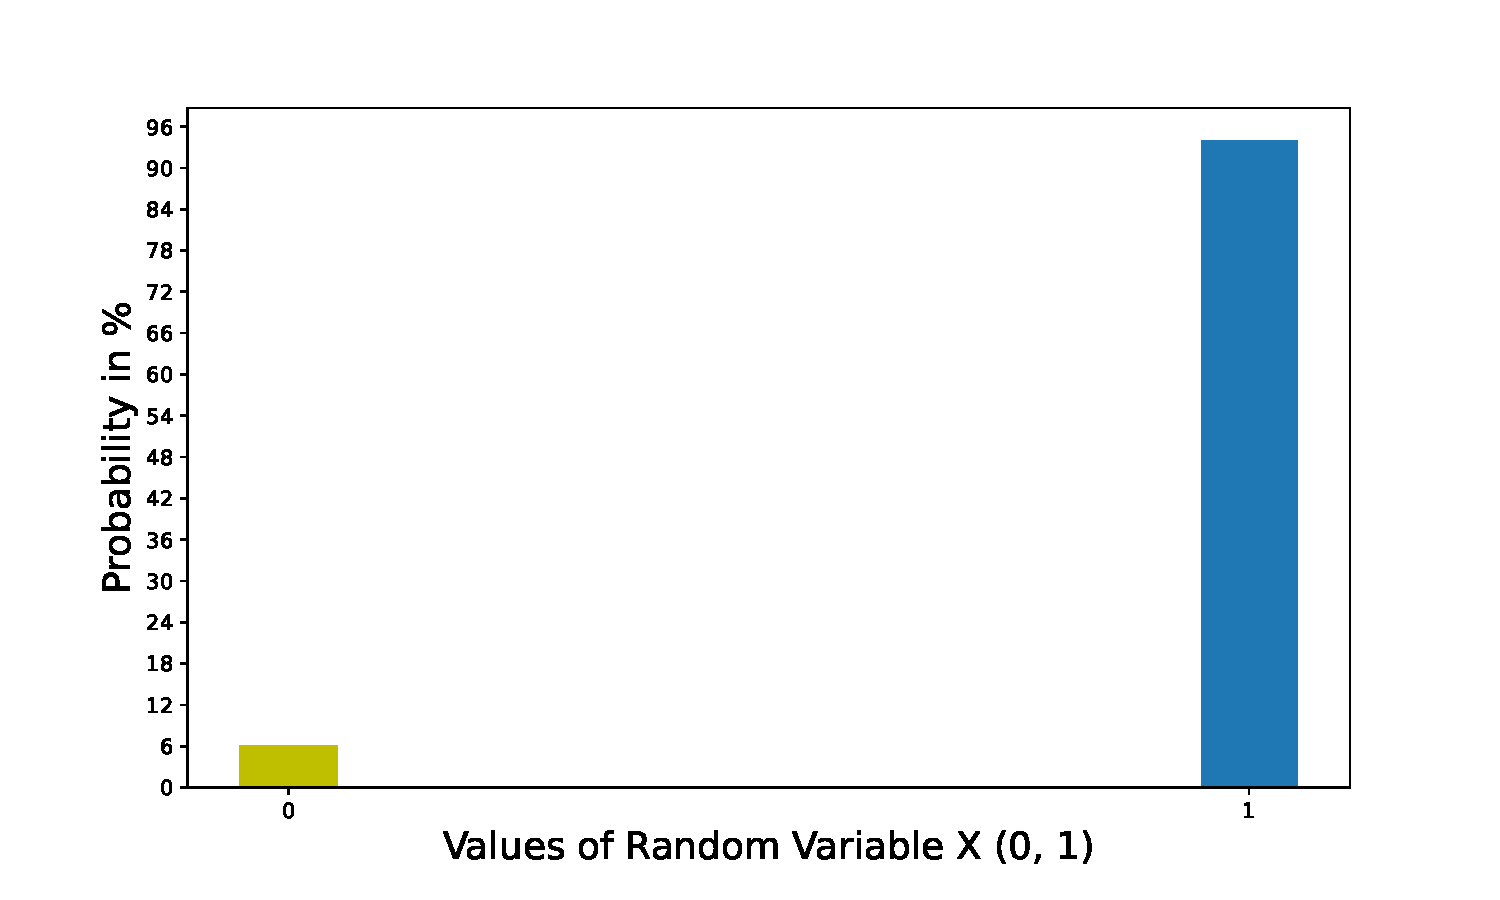
\includegraphics[width=17cm]{pics/task_1_a.pdf}
\caption{Bernoulli’s single trial P (votes=for & votes = against)}\label{fig:task_1_a}
\end{figure}
\FloatBarrier

\newpage

\begin{lstlisting}[caption={: Plotting the PMF for representing Bernoulli’s single trial P (votes=for & votes = against)},label=code_task_1_a]
from scipy.stats import bernoulli
import matplotlib.pyplot as plt

p = 0.27
# The result of the random variable is either yes or no, i.e. 0 and 1 for a Bernoulli's experiment.
X = [0, 1]

# pmf of the bernoulli single trial in %
pmf_bd_in_percent = bernoulli.pmf(X, p) * 100

# Plot the probability distribution
fig, ax = plt.subplots(1, 1, figsize=(10, 6))

plt.xlabel("Values of Random Variable X (0, 1)", fontsize="18")
plt.ylabel("Probability in %", fontsize="18")
bar_list=plt.bar(X, pmf_bd_in_percent, width=0.1)
bar_list[0].set_color('y')
plt.xticks([0,1, 1])

plt.savefig('images/task_1_a.pdf')
\end{lstlisting}

\section{Task b}

A Poisson distribution is mainly used to describe discrete random variable X which gives the probability of several independent events observed over a fixed interval of time, i.e., number of people entering a supermarket in a Saturday each hour. \newline

The event of meteorites falling on the ocean each year also follows a similar pattern with the supermarket example, where the falling meteorites (discrete independent events) are observed over a year with an expectation ${\lambda}$=37. Since this random event is also observed a certain number of times in a defined time interval, we can say that Poisson is a natural candidate for such a phenomenon.\newline

In Figure \ref{fig:task_1_b} we can see that the number of meteorites (n) which can fall in a year is chosen to be 53 in the distribution. Looking at the probabilities  \begin{equation} P(X=k)=\frac{\lambda^k e^{-k}}{k!}, k=0,1,2…,  \label{pmf_poission}\end{equation} when k=52 the probability of meteorites falling is less than 0.5 or 0.005. Due to this reason the n=52 is used to depict the distribution. 

\subsubsection{Median and Variance}
The variance of a Poisson distribution is given by Var[X]=$\lambda=\sigma^2$ (\cite{hogg:2005}), therefore the variance of this distribution is equal to λ parameter Var[X]=37.
Likewise, the median can be defined as the mid-point, where 50\% of the samples are either above or below this point. For this we can calculate the value of X whose cumulative sum of the probability is less than 50\%. In this case the median is 37 which is the same as the median and variance $\lambda$. The calculation of the median or 2nd quartile is done using a for loop see (listing \ref{lst:code_task_1_b} line 21)  with the cumulative sum of the probabilities and the median is stored when a value is found which is greater than 50 is found. Therefore, we can say that for this distribution the mean, median and variance are the same.

\begin{lstlisting}[caption={Plotting the PMF for Poisson Distribution)},label={lst:code_task_1_b}]
from scipy.stats import bernoulli
import matplotlib.pyplot as plt

from scipy.stats import poisson
import numpy as np
import matplotlib.pyplot as plt

# Definitions
tick_increment = 1
lmbda = 37
n = 53
X = np.arange(0, n, 1)

mean, var, skew, kurt = poisson.stats(lmbda, moments='mvsk')

# PMF of the distribution in %
poisson_pd = poisson.pmf(X, lmbda) * 100

#Finding variance by summing the pdf  to get CDF
median = 0
for i , e in enumerate(poisson_pd.cumsum()):
    if e > 50:
        median = i
        print(i)
        break


p_lmbda = poisson.pmf(k=var, mu=lmbda) * 100
p_median = poisson.pmf(k=median, mu=lmbda) * 100

# Plot the probability distribution
fig, ax = plt.subplots(1, 1, figsize=(20, 6))

#ax.plot(X, poisson_pd, 'bo', ms=10, label='poisson pmf')
#PMF
plt.xlabel("X - No. of Meteorites", fontsize="18")
plt.plot(X, poisson_pd, 'bo', ms=10, label='poisson pmf')
ax.vlines(X, 0, poisson_pd, colors='b', lw=5, alpha=0.5)

#Variance
plt.plot(var, p_lmbda, 'co', ms=10, label='Variance')
ax.vlines(var, 0, p_lmbda, colors='c', lw=5, alpha=0.5)

#Median
plt.plot(median, p_median, 'ro', ms=10, label='Median')
ax.vlines(median, 0, p_median, colors='r', lw=5, alpha=0.5)

plt.xticks(np.arange(0, n, tick_increment))
plt.title("Poisson Distribution - No. of Meteorites λ = 37", fontsize="18")

plt.ylabel("Probability in %", fontsize="18")
ax.grid(True)

plt.legend(loc='best', frameon=True)
plt.savefig('images/task_1_b.pdf')

\end{lstlisting}

\begin{figure}[h!]
\centering
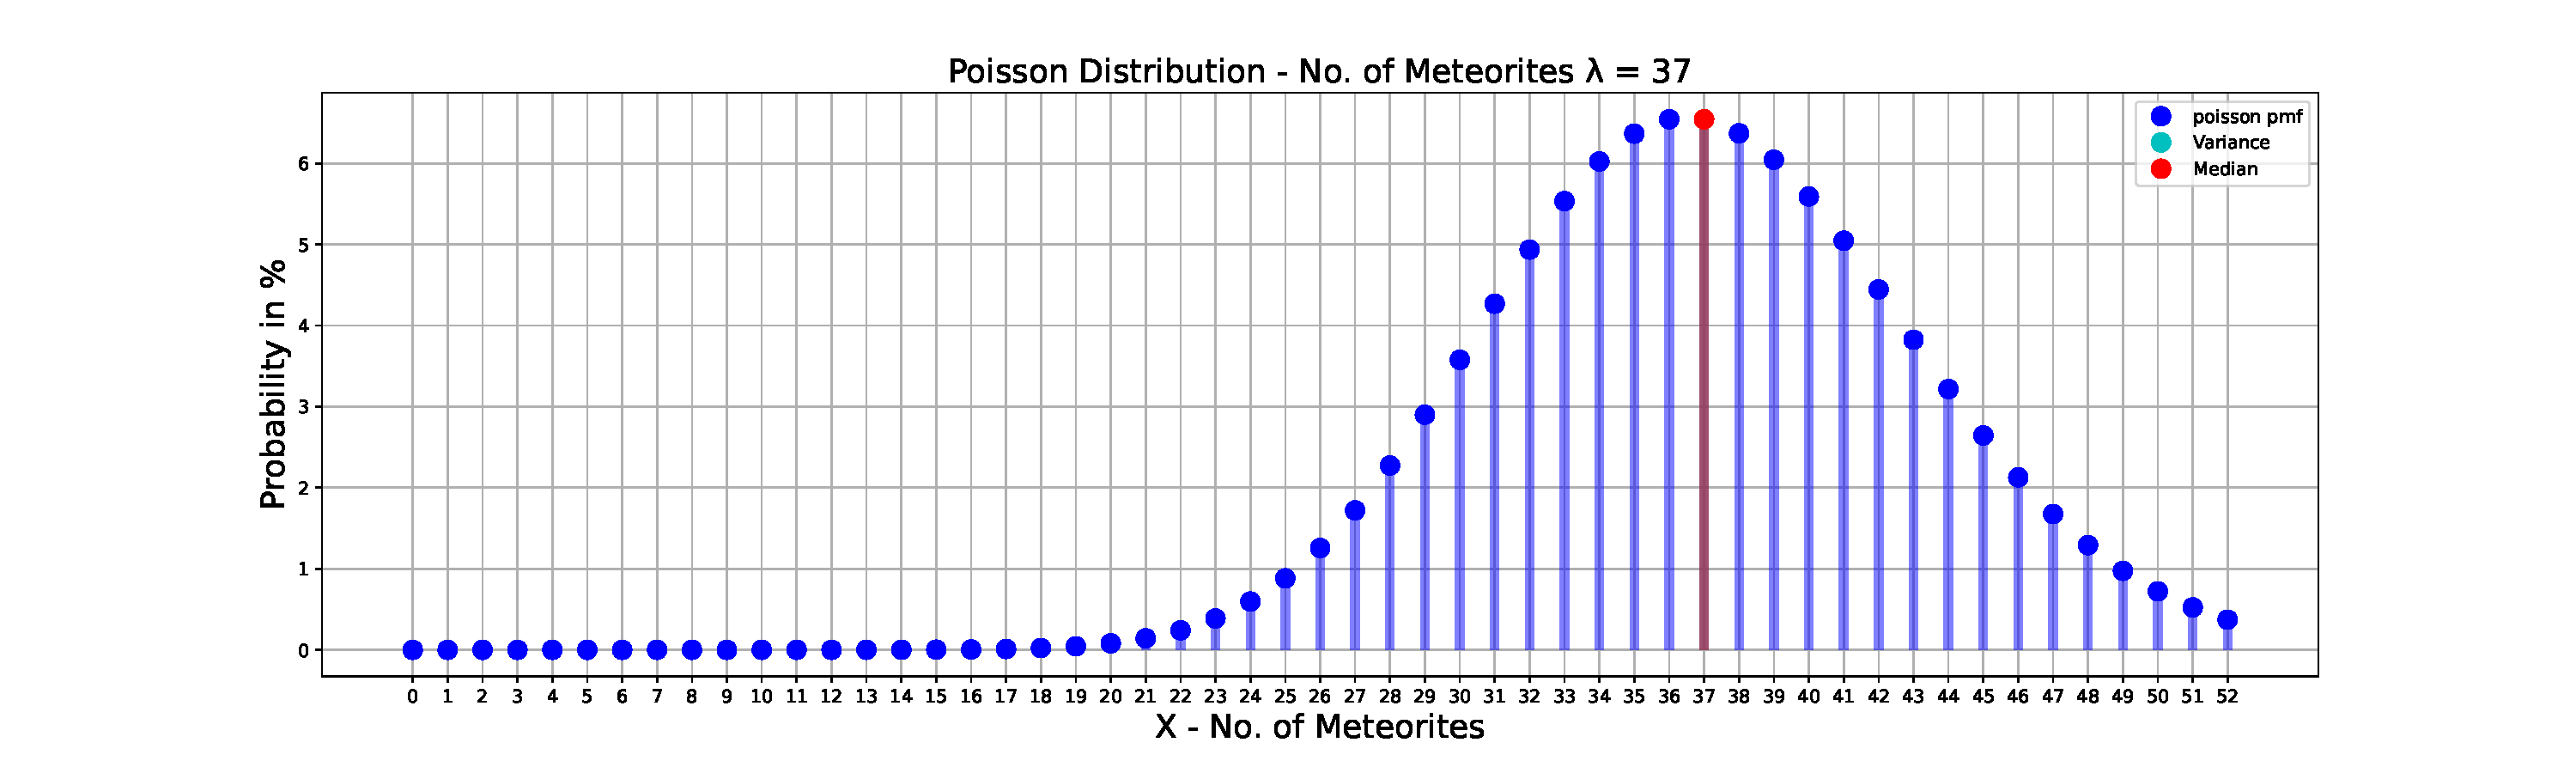
\includegraphics[width=\textwidth]{pics/task_1_b.pdf}
\caption{Poisson Distribution with n = 53 with median and variance}\label{fig:task_1_b}
\end{figure}
\FloatBarrier

\section{Task c}

Given that Y is a random variable with time to hear an owl, and the probability ones needs to wait to hear the owl after y hours is:
\begin{equation} \label{eqn:cdf_minus_1}
    P(Y > y) = 0.3e^{-0.5y} + 0.7e^{-0.25y} (Rounded up)
\end{equation}
Since the probability given is the probability of hearing the owl after y hours is the complementary cumulative distribution function (CCDF) P(Y $>$ y), the CDF would be 1 minus the equation \ref{eqn:cdf_minus_1} (\cite{Iubh:2021}, pg.89). The CDF is as follows:
\begin{equation} \label{eqn:cdf}
    P(Y\leq y) = F(x) = 1 -(0.3e^{-0.5y} + 0.7e^{-0.25y})
\end{equation}
We can obtain the probability density function by taking the first derivative of the Cumulative distribution function. The steps for the derivative are below: 
\begin{enumerate}
    \item $f(y) = \frac{\partial F}{\partial y}$
    \item $f(y)= 1- (0.3e^{-0.5y} + 0.7e^{-0.25y})  \frac{\partial F}{\partial y}$
   \item $f(y)= -(0.3e*-0.5e^{-0.5y} + 0.7-*0.25e^{-0.25y})  \frac{\partial F}{\partial y}$ 1 is removed because it is a constant
   \item $f(y)= (0.15e^{-0.5y} + 0.175e^{-0.25y})$\label{eqn:pdf_exp}
\end{enumerate}
    Therefore the PDF of the function is
\begin{equation}\label{eqn:pdf_owl}
    f(y) =\begin{cases*}
    0.15e^{-0.5y} + 0.175e^{-0.25y}&\text{for y$>$0}
    &\\0&\text{elsewhere}
    \end{cases*} \newline
\end{equation}
Additionally, the probability of hearing the owl lies in between the limits (2, 4] and calculated using the difference of the Probability of hearing an owl at 4 hours and 2 hours, which is as follows:

\begin{equation}
 P(2< Y \le 4) = F_{Y}(4) - F_{Y}(2)   
\end{equation}
The steps for the calculations are as follows:
\begin{enumerate}
    \item $ P(2< Y \le 4) = F_{Y}(4) - F_{Y}(2)$
    \item $ P(2< Y \le 4) = 0.70 - 0.47$
    \item $ P(2< Y \le 4) = 0.23$
\end{enumerate}
    
\subsubsection{Median Variance \& Quartiles}    

The mean μ can be calculated using E[Y]= $\mu$= $\int_{-\infty}^{\infty} yf(y)\,dy$. The density function f(y) used can be found in equation (\ref{eqn:pdf_owl}). Accordingly, the steps to calculate the mean are as follows: 

\begin{enumerate}
    \item E[Y] = $\int_{-\infty}^{\infty} yf(y)\,dy$
    \item E[Y] = $\int_{0}^{\infty} yf(y)\,dy$.  We can change the limits from $-\infty$ to 0 because there exists no value before 0.
    \item E[Y] = $\int_{0}^{\infty} y(0.15e^{-0.5y} + 0.175e^{-0.25y})\,dy$.
    \item E[Y] = $\int_{0}^{\infty} 0.15ye^{-0.5y} + \int_{0}^{\infty} 0.175ye^{-0.25y}\,dy$.
    \item E[Y] = $\int_{0}^{\infty} 0.15ye^{-0.5y} + \int_{0}^{\infty} 0.175ye^{-0.25y}\,dy$ \label{eqn:mean_line_5}
    \item E[Y] = $[0.15(-2ye^{-0.5y}-4e^{-0.5y})]_0^\infty + [0.175(-4ye^{-0.25y}-16e^{-0.25y})]_0^\infty$ Using integration by parts formula
    \item E[Y] = $[(-0.3ye^{-0.5y}-0.6e^{-0.5y})]_0^\infty + [-0.7ye^{-0.25y}-2.8e^{-0.25y})]_0^\infty$
    \item E[Y] = $[\lim_{b\to\infty}(0)-(-0.3*0e^{-0.5*0}-0.6e^{-0.5*0})] + [\lim_{b\to\infty}(0)-(-0.7*0e^{-0.25*0}-2.8e^{-0.25*0})]$ Applying the limits.
    \item E[Y] = 3.4
\end{enumerate}
Therefore the expectation of the function E[Y]=$\mu$=3.4. Similarly, the variance can be calculated using the following formula Var[Y]= $\int_{-\infty}^{\infty}y^2f(y)\,dy - \mu^2$. The steps to calculate the variance are as follows: 


\begin{enumerate}
    \item E[$Y^2$] = $\int_{-\infty}^{\infty}y^2f(y)\,dy$
    \item E[$Y^2$] = $\int_{0}^{\infty} y^2f(y)\,dy$.  We can change the limits from $-\infty$ to 0 because there exists no value before 0.
    \item E[$Y^2$] = $\int_{0}^{\infty} y^2(0.15e^{-0.5y} + 0.175e^{-0.25y})\,dy$.
    \item E[$Y^2$] = $\int_{0}^{\infty} 0.15y^2e^{-0.5y} + \int_{0}^{\infty} 0.175y^2e^{-0.25y}\,dy$.
    \item E[$Y^2$] = $\int_{0}^{\infty} 0.15ye^{-0.5y} + \int_{0}^{\infty} 0.175ye^{-0.25y}\,dy$
    \item E[$Y^2$] = $[0.15(-2y^2e^{-0.5y}+4\int ye^{-0.5y})]_0^\infty + [0.175(-4y^2e^{-0.25y}+8\int ye^{-0.25y})]_0^\infty$ Using integration by parts formula. see above line (\ref{eqn:mean_line_5}), the integration is has been already done in the step and will copy the part here.
    \item E[$Y^2$] = $[0.15(-2y^2e^{-0.5y} +4(-2ye^{-0.5y}-4e^{-0.5y})]_0^\infty + [0.175(-4y^2e^{-0.25y} +8(-4ye^{-0.25y}-16e^{-0.25y})]_0^\infty$
    \item E[$Y^2$] = $[0.15(\lim_{b\to\infty}(0)-(-2*0^2e^{-0.5*0} +4(-2*0e^{-0.5*0}-4e^{-0.5*0})] + [0.175(\lim_{b\to\infty}(0)-((-4*0^2e^{-0.25*0} +8(-4*0e^{-0.25*0}-16e^{-0.25*0})]$
    \item E[$Y^2$] = 0.15*16+ 0.175*128 = 2.4 + 22.4 = 22.8
    \item Var[Y] = E[$Y^2$] - $\mu^2$ = 22.4 + $3.4^2$ = 13.24 \label{eqn:var_task_1_c}
\end{enumerate}

As calculated in line \ref{eqn:var_task_1_c} the variance Var[Y] = 13.24. To find the quartiles one can use again the CDF, and compare it with the value of x using this the Q1(25\%) = 0.92 , Q1(50\%) = 2.23 and Q1(75\%) = 4.63. Alternatively, one can use the inverse of the CDF $F_{Y}^{-1} (.)=x$ to also find the given quartile.

\begin{figure}[h!]
\centering
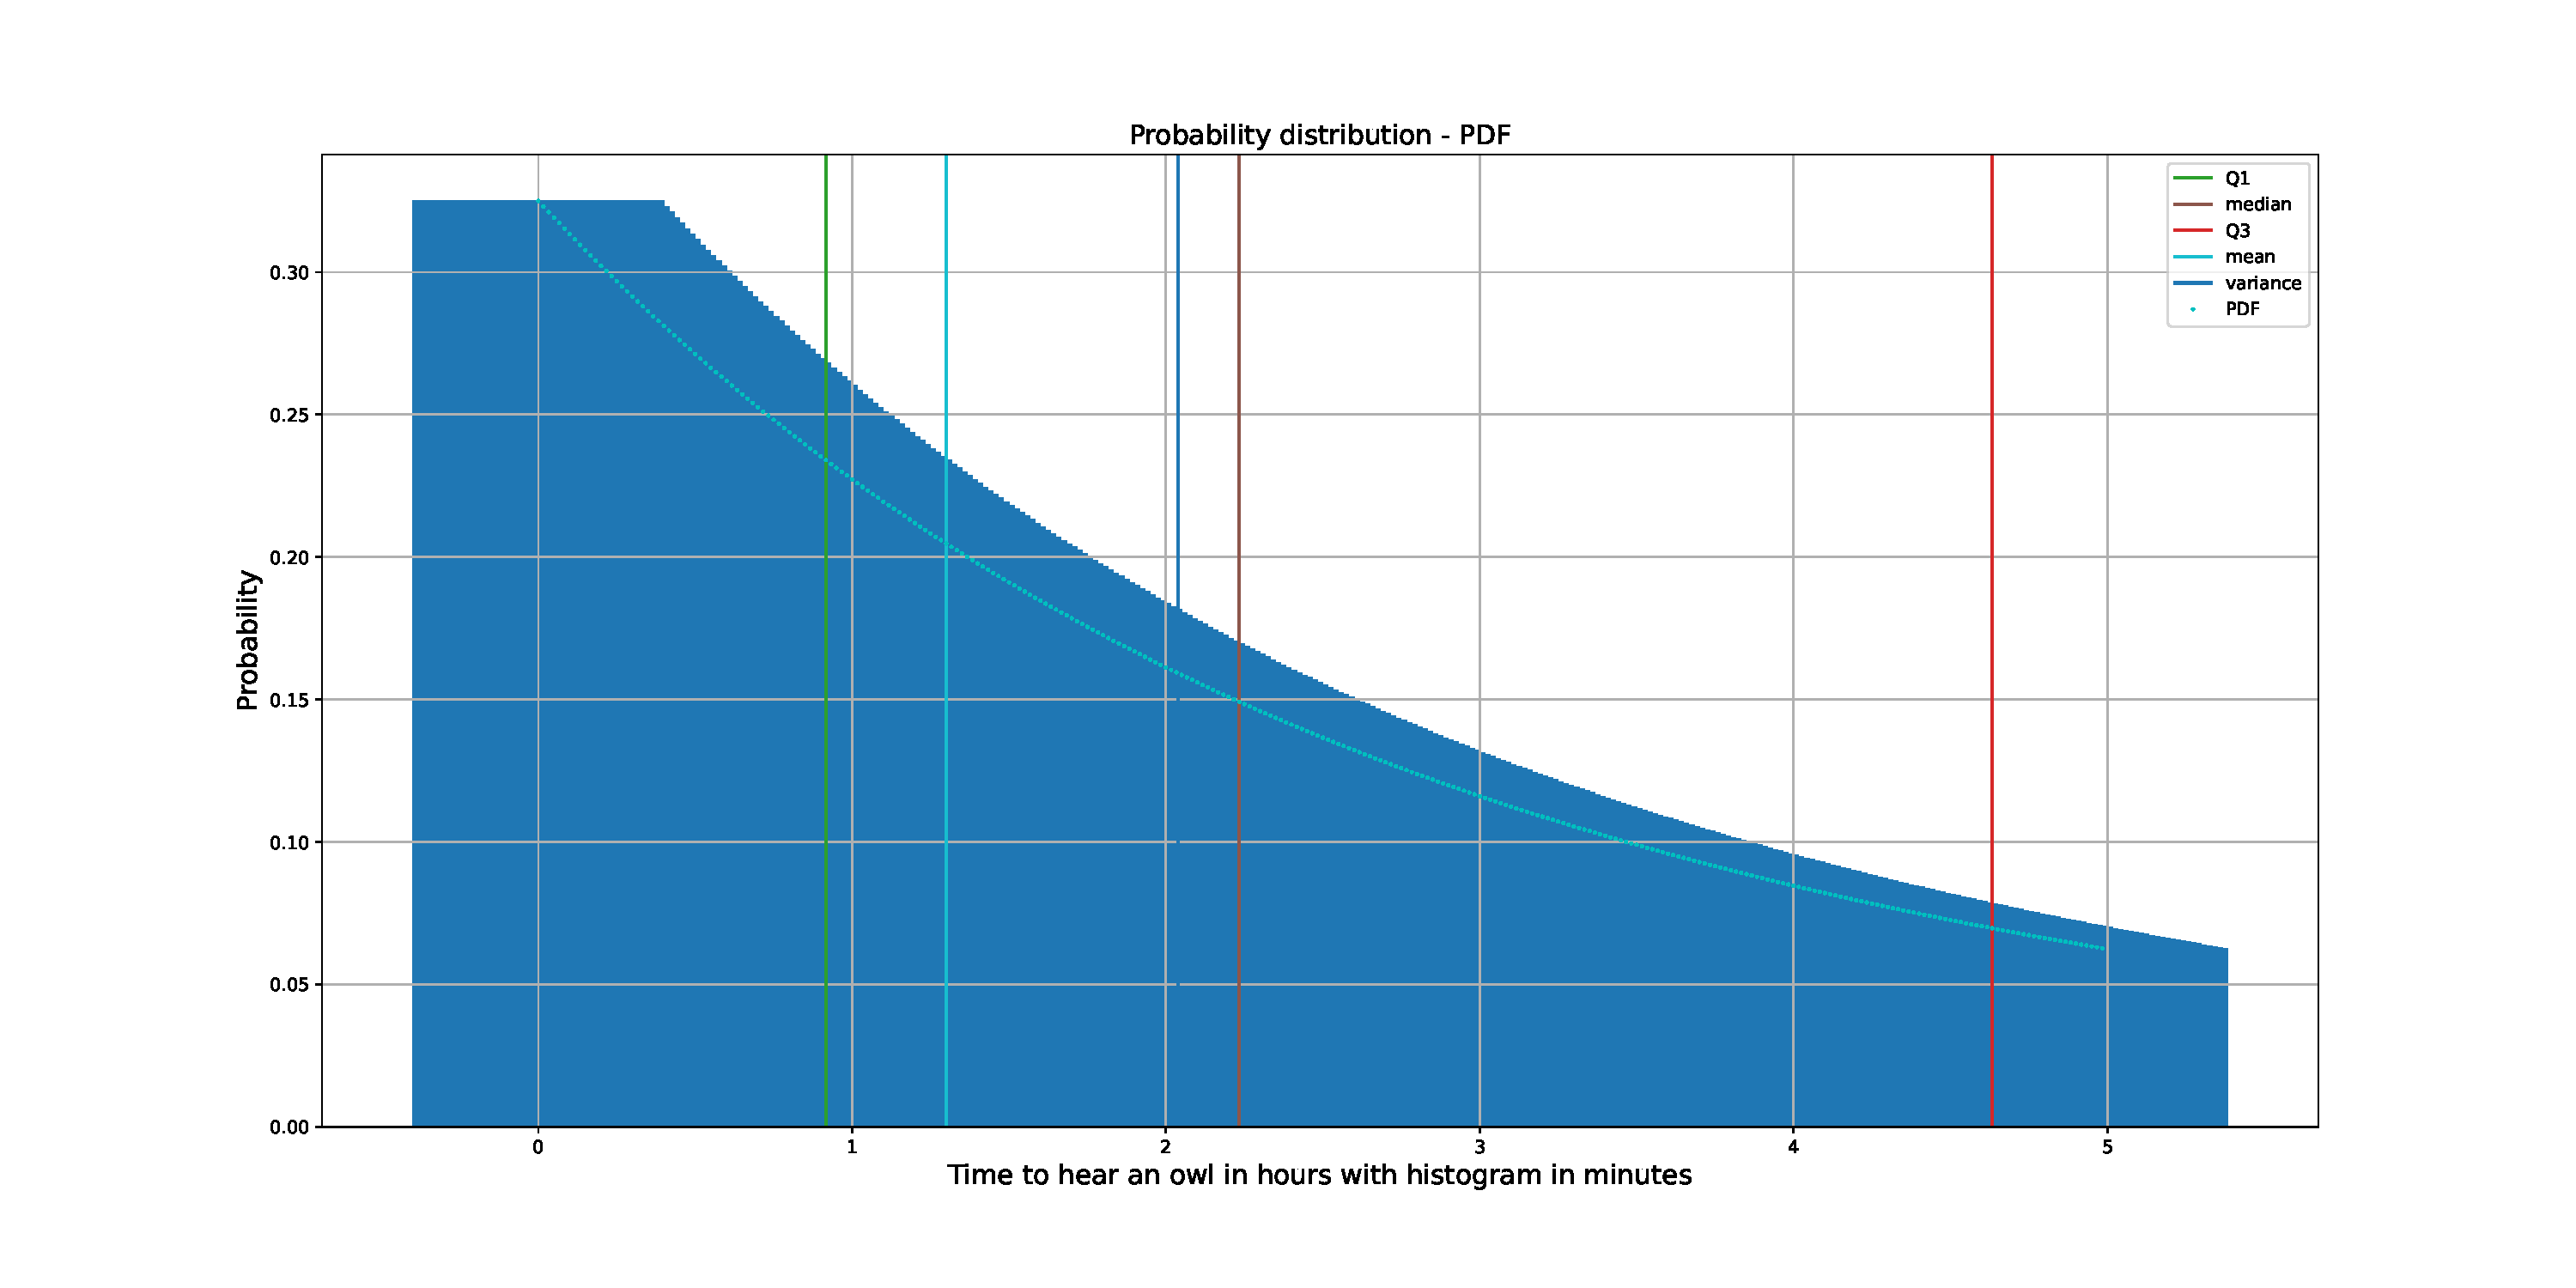
\includegraphics[width=\textwidth]{pics/task_1_c_pdf.pdf}
\caption{PDF for time to wait to hear an owl with histogram per minute (5h)}\label{fig:task_1_c}
\end{figure}
\FloatBarrier    


\begin{lstlisting}[caption={Plotting the PDF and histogram)},label={lst:code_task_1_c}]

import numpy as np
import matplotlib.pyplot as plt
from scipy.stats import rv_continuous

title_pdf = 'Probability distribution - PDF'
title_hist = r'Histogram by Minute(width = $\frac{1}{60}$  = 0.017)'
n = 5
start = 0
tick_increment = (1/60)

def my_pdf(y):
    return np.exp(y * -0.5) * 0.15 + np.exp(-0.25 * y) * 0.175

def my_cdf(y):
    return 1 - (np.exp(y * -0.5) * 0.3 + np.exp(-0.25 * y) * 0.7)

def my_ccdf(y):
    return 1 - (np.exp(y * -0.5) * 0.3 + np.exp(-0.25 * y) * 0.7)

def calc_quartile(quartile, cdf_val, x_vals):
    #Finding variance by the CDF 
    for index , val in enumerate(cdf_val):
        if val > quartile:
            return x_vals[index]
            break

# generate data by the minute
x = np.arange(0, n, tick_increment)
my_distribution = my_dist()
p = my_pdf(x)
cdf = my_cdf(x)

#PDF
fig, ax = plt.subplots(1, 1, figsize=(20, 10))
ax.set_title(title_pdf, fontsize=15)
ax.set_xlabel('Time to hear an owl in hours with histogram in minutes', fontsize=15)
ax.set_ylabel('Probability', fontsize=15)


# Label pdf
plt.axvline(calc_quartile(0.25, cdf, x), label='Q1', c='tab:green', linestyle='solid')
plt.axvline(calc_quartile(0.5, cdf, x), label='median', c='tab:brown', linestyle='solid')
plt.axvline(calc_quartile(0.75, cdf, x), label='Q3', c='tab:red', linestyle='solid')
plt.axvline(1.3, label='mean', c='tab:cyan', linestyle='solid')
plt.axvline(2.04, label='variance', c='tab:blue', linestyle='solid')

plt.bar(x, p)
plt.plot(x, p, 'co', ms=1, label='PDF')
ax.grid(True)
plt.legend(loc='best', frameon=True)
plt.savefig('images/task_1_c_pdf.pdf')
\end{lstlisting}



\chapter{Assignment 2: Basic Probabilities and Visualizations}

\section{Task a}
For the given samples (Variable X and Y) a scatter plot deems to be the most suitable candidate to plot the given points. This can be said because scatter plot helps to show the relationship between two variables, as one can see where the different points lie in the graph. This tells us how co-related the samples are.

\begin{figure}[h!]
\centering
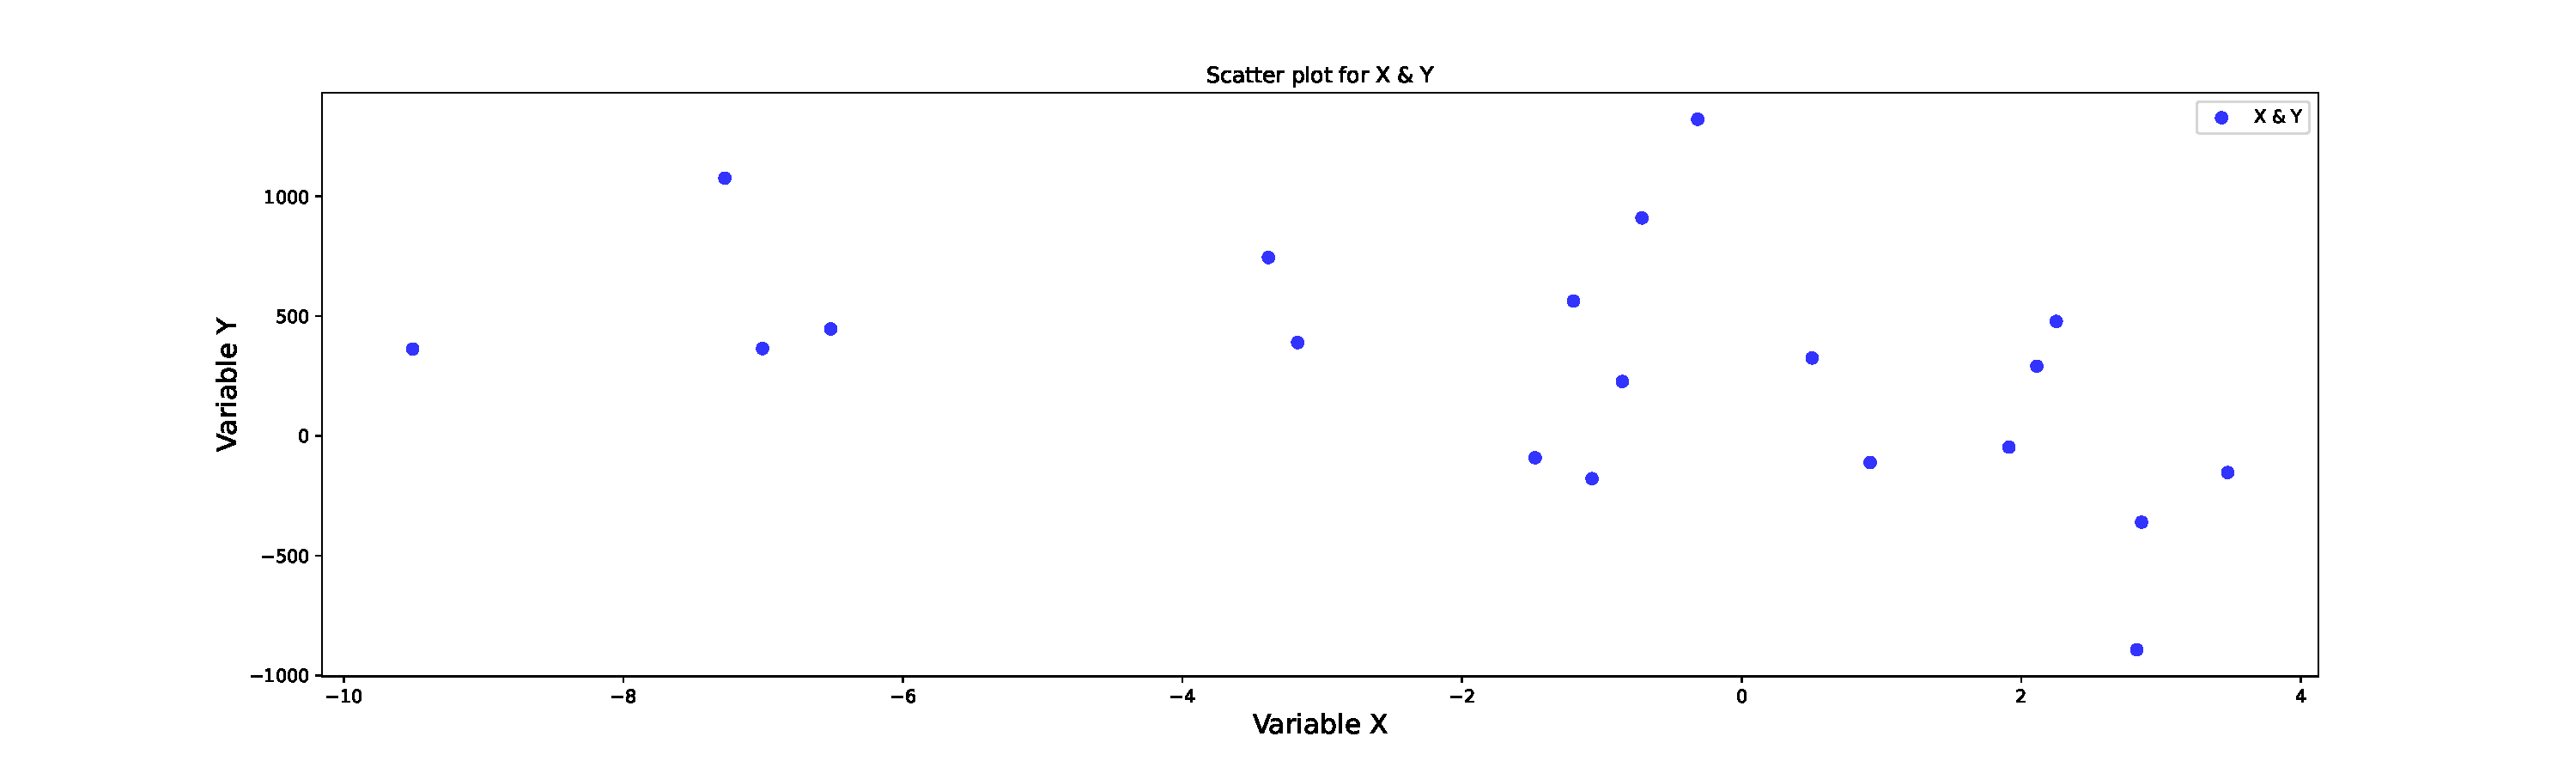
\includegraphics[width=\textwidth]{pics/task_2_a.pdf}
\caption{Scatter Plot for X and Y}\label{fig:task_2_a}
\end{figure}
\FloatBarrier
\newline 
A simple look in the scatter plot (fig:\ref{fig:task_2_a}) shows us the data have a very large covariance as the points in the graph are very sparsely distributed in the plot.

\begin{lstlisting}[caption={Plotting the Scatter Plot with Variance Calculations)},label={lst:code_task_2_a}]
import numpy as np
import matplotlib.pyplot as plt

# Definitions
sample_data = [(-1.202, 563.024), (2.112, 291.072), (2.827, -893.619), (-0.314, 1321.814),
               (-1.477, -91.573), (-6.516, 446.336), (0.920, -111.487), (3.477, -153.165),
               (-7.273, 1076.221), (2.251, 477.931), (-0.713, 909.696), (-0.853, 226.865),
               (-3.176, 389.413), (1.913, -47.169), (-1.070, -178.695), (-3.385, 744.486),
               (-9.506, 362.670), (-7.004, 364.578), (0.504, 324.975), (2.861, -360.571)]

# Plot the probability distribution
fig, ax = plt.subplots(1, 1, figsize=(20, 6))
# Separate value of X and Y from sample data
x, y = zip(*sample_data)

plt.scatter(x, y, color='b', label='X & Y', alpha=0.8)
plt.title('Scatter plot for X & Y')
plt.xlabel('Variable X', fontsize=15)
plt.ylabel('Variable Y', fontsize=15)

# Mean and covariance
mean_x = sum(x) / len(x)
mean_y = sum(y) / len(y)
x_minus_mean_x = np.asarray(x) - mean_x
y_minus_mean_y = np.asarray(y) - mean_y
# Covariance of X & Y
cov_x_y = sum(x_minus_mean_x * y_minus_mean_y) / len(x)
# Variance of X
var_x = sum(np.power(x_minus_mean_x, 2)) / len(x)
# Variance of Y
var_y = sum(np.power(y_minus_mean_y, 2)) / len(y)

plt.legend()
plt.savefig('images/task_2_a.pdf')
\end{lstlisting}

\subsubsection{Mean \& Covariance}   

The mean of Variables can be calculated using E[X]=  $\frac{1}{N} \sum_{i=1}^{N}x_i$  (\cite{Iubh:2021}) where N=20 is the total number of samples and the numerator is the sum of the random variable X or Y. Using this formula, the expectation ($\mu$) of the variable X and Y are calculated. E[X] = $\mu_x$= -1.28 and E[Y] = $\mu_y$= 283.14.\newline 
The Covariance of two variables can be calculated using cov(X,Y) =  $\frac{1}{N} \sum_{i=1}^{N}(x_i - \mu_x)^2 (y_i - \mu_y)$ (\cite{Iubh:2021}). Using the given formula, the cov(X,Y)= -863.73

Similarly, the Variance can be calculated using var[X]=$\frac{1}{N} \sum_{i=1}^{N}(x_i - \mu_x)^2$. The calculated variances are as follows Var[X]=13.60 and Var[Y]= 2.6e+5.

\subsection{Task b}

\chapter{Assignment 3: A Simple Parameter Estimation}

Given, is a density function of a random variable S which is a type of network router with a bandwidth total to first hardware failure dependent on a single unknown parameter $\theta$ and T is the bandwidth total to failure of the sequence of two routers. Also, the density for the random variable S is assumed to be modeled using an exponential distribution s(t)=  $\frac{1}{\theta} \exp{\frac{-t}{\theta}}$ . As T can be defined as the sum of the density functions of the two routers $S_1$  and $S_2$, we can express the density function of  $T= S_1+S_2$.\newline \newline 
We can assume that the variables $S_1,S_2$,…,$S_n$ are independent and identically distributed. It can also be called an independent and identically distributed variable because the bandwidth total to failure of one router would not affect the other. Additionally, we can assume that the density function of the random variable is a continuous function, as it is modelled by an exponential function.\newline \newline
Using the assumptions and using the transformation theorem (\cite{Iubh:2021}, pg. 97), we can calculate the sum of the two density functions $S_1$  and $S_2$ by convolving them, which can be also written in a short form as $T=S_1*S_2= \int_{-\infty}^{\infty} S_1(T-\tau) S_2(\tau) \,d\tau\ $.\newline\newline
We can further simply the limits of the integral which start only from 0 because the flipped function does not overlap until it reaches 0 and then it only overlaps until t when it shifts so the convolution equation can be simplified as$T=S_1*S_2= \int_{0}^{t} S_1(T-\tau) S_2(\tau)\,d\tau\ $.The steps for calculating the density function of T are as follows:

\begin{enumerate}
    \item $ T = \int_{0}^{t} S_1(T-\tau) S_2(\tau)\,d\tau\ $
    \item $ T = \int_{0}^{t} \frac{1}{\theta} e^{\frac{-(t-\tau)}{\theta}} \frac{1}{\theta} e^{\frac{-t}{\theta}}\,d\tau\ $
    \item $ T = \frac{1}{\theta^2}\int_{0}^{t} e^{\frac{-t+\tau}{\theta}} e^{\frac{-t}{\theta}}\,d\tau\ $
    \item $ T = \frac{1}{\theta^2}\int_{0}^{t} e^{\frac{-t+\tau-\tau}{\theta}}\,d\tau\ $
    \item $ T = \frac{1}{\theta^2}\int_{0}^{t} e^{\frac{-t}{\theta}}\,d\tau\ $
    \item $ T = \frac{1}{\theta^2} e^{\frac{-t}{\theta}}\int_{0}^{t} 1\,d\tau\ $ The exponential can be taken out because there is no dependence on $\tau$.
    \item $ T = \frac{1}{\theta^2} e^{\frac{-t}{\theta}}[\tau]_{0}^{t} $
    \item $ T = \frac{1}{\theta^2} e^{\frac{-t}{\theta}}(t-0) $ Replacing $\tau$ with the limits we
    calculated the density of T.
    \item $ T = \frac{1}{\theta^2} e^{\frac{-t}{\theta}}t$
\end{enumerate}

The calculated density function of T is 
\begin{equation}\label{eqn:pdf_T}
    f(y) =\begin{cases*}
    \frac{1}{\theta^2} e^{\frac{-t}{\theta}}t &\text{for y$>$0} 
    &\\0 &\text{elsewhere}
    \end{cases*} \newline
\end{equation}
Using the density function of T, we can also calculate the likelihood function which is: 

\begin{enumerate}
    \item $ f(\theta/T) = \prod_{i=1}^{n} \frac{1}{\theta^2} e^{\frac{-t_i}{\theta}}t_i,  \forall_i \in {1,2,... n}, t_i \in [0, \theta]$
    \item $ f(\theta/T) = \frac{1}{\theta^{2n}} e^{-\sum_{i=1}^{n} \frac{t_i}{\theta}} \prod_{i=1}^{n} t_i $. Simplifying the equation.
\end{enumerate}
So, the calculated likelihood function is $ f(\theta/T) = \frac{1}{\theta^{2n}} e^{-\sum_{i=1}^{n} \frac{t_i}{\theta}} \prod_{i=1}^{n} t_i $. This function can be transformed by using log, as the multiplications can be converted into sums which would be easier to calculate. The transformed likelihood function is $l(\theta) = log(\frac{1}{\theta^{2n}} + log(e^{-\sum_{i=1}^{n} \frac{t_i}{\theta}}) + log(\prod_{i=1}^{n} t_i)$. Using the transformed likelihood function we can calculate the maximum likelihood function for $\theta$ by finding the first derivative of the log function where the slope is 0.

\begin{enumerate}
    \item $ \frac{dl}{d\theta} = log(\frac{1}{\theta^{2n}} + log(e^{-\sum_{i=1}^{n} \frac{t_i}{\theta}}) + log(\prod_{i=1}^{n} t_i)$
    \item $ \frac{dl}{d\theta} = log(1) - 2n log(\theta) + log(e^{-\sum_{i=1}^{n} \frac{t_i}{\theta}}) + log(\prod_{i=1}^{n} t_i)$
    \item $ \frac{dl}{d\theta} =- 2n log(\theta) + log(e^{-\sum_{i=1}^{n} \frac{t_i}{\theta}}) + log(\prod_{i=1}^{n} t_i)$
    \item $ \frac{dl}{d\theta} =\frac{-2n}{\theta} - {\sum_{i=1}^{n} \frac{t_i}{\theta^2}}+0$. The derivative with no dependence to $\theta$ is 0
    \item $ 0 =\frac{-2n}{\theta} - {\sum_{i=1}^{n} \frac{t_i}{\theta^2}}$
    \item $ \theta_{MLE} ={\sum_{i=1}^{n} \frac{t_i}{2n}}$
\end{enumerate}
The computed maximum likelihood of the bandwidth to total with the given data from the experiment is $T_{MLE}={\sum_{i=1}^{n} \frac{t_i}{2n}} = \frac{56}{10} =5.6$ and the expectation is E[T] = $\sum_{i=1}^{n} \frac{t_i}{n} = \frac{56}{5} = 11.2$.
%\chapter{Latex}

\section{Tools}

MiKTeX: \url{https://miktex.org/download}
TeXLive: \url{http://tug.org/texlive/}
 (or alternative LaTeX-systems).
 
 A good editor is essential. Sometimes combined editors and compilers (e.g. TeXShop) can be really productive. Make sure you learn the use of synchronized navigation then.

A vector graphic is one where strokes remain strokes even at the highest resolutions: e.g. the Figure~\ref{fig:spiral} or the Logo on the \hyperref[titlePage]{Titelblatt} (notice: you can click from here to there).
Many tools generate vector-graphics for plots from any data-set. E.g. Plotly (with the use of the Browser-Print), MatPlotLib or even OpenOffice, LibreOffice or MS-Excel.

\section{Literature References}
Here is an example of a reference with a page-number: \cite[S. 6]{DueckKo:2016}


\section{Pictures}

\begin{figure}[h]
\centering
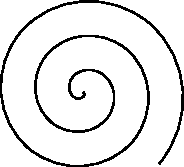
\includegraphics[width=8cm]{pics/spiral.pdf}
\caption{A spiral... smooth vector-based with a clean parametrisation! \\ Nothing to do with \cite{Gage:18}}\label{fig:spiral}
\end{figure}
\FloatBarrier

\section{Tables}

\begin{table}[H]
\small
\centering
\begin{tabular}{p{5cm}|l|p{3cm}}
`` Industrial era '' &  ``Jobs '' & `` Wanted: Upgrade''' \\ \hline
Parts exchanger & Fitter & mecatronics specialist \\
eShop & reseller & `` Client-suggester'' \\
`` Coding-guru''' & Softwaredesign & Whole-life designer \\
JA! Gut \& Günstig & brand-names & `` Life-Style Feeling'' \\
Internetbanking & Bank clerk & Customer adviser \\
Robots & Specialist & Machine supervisor \\
Bush & Gardener & Nature-sculptor \\
Painting & Painter & Interior Design \\
 &  & \\
\end{tabular}
\caption[Downgrade and upgrade of job denominations]{Downgrade and Upgrade of job denominations \\ \ \ \ \cite{DueckKo:2016}}
\label{tab:Downgrade and Upgrade of job denominations}
\end{table} 

\section{Listes}

\begin{itemize}
 \itemsep0pt
 \item one
 \item twoi
 \item threei
\end{itemize}

\begin{enumerate}
 \itemsep0pt
 \item first
 \item second
 \item third
\end{enumerate}


\section{Formulæ}

A formula can be written inline, e.g. as $ \frac{d}{dx}\mbox{arctg}(x) = \frac{1}{1+x^2}$ or, in centered math:

\begin{equation}  \frac{d}{dx}\mbox{arctg}(x) = \frac{1}{1+x^2} \label{arctanderivative}\end{equation}

Notice that formulæ that are centered start bigger (technically, they start in \verb+\displaystyle+) than they start inline (technically, they start in \verb+\textstyle+ all subsequents reductions, e.g. an exponent, goes to \verb+\scriptstyle+ then \verb+\scriptscriptstyle+). Indeed a best effort is made so that inline formulæ do not change the line height which would bother the eye of a reader.

Formulæ can be given a number and a label. Numbering happens automatically with \verb+\begin{equation}+ and \verb+\end{equation}+ and can be avoided if enclosing the formula betwee \verb+\[+ and \verb+\]+. If using the \verb+\label+ macro inside, you can refer automatically to this equation using \verb+\ref{label}+. E.g. Thanks to equation~\ref{arctanderivative} one dare say that:

\begin{equation} \int_0^t \frac{1}{1+x^2} dx = \mbox{arctan}(t) \end{equation}


\section{Tools and Code}

Many users of this template will want to include some code.

The simplest way to do so is to use the \verb+\verb+ macro which is followed by a sign, then some code, then the sign again to close. This is the inline version which works as in: 


\begin{verbatim}
As we could calculate with \cite{Wolfram_alpha} using 
\verb_integrate 1 / pi e ^ (t/pi) from zero to infinity_.
\end{verbatim}

which yields: 

As we could calculate with \cite{Wolfram_alpha} using \verb_integrate 1 / pi e ^ (t/pi)_ from zero to infinity.


The multiline version of this is called \verb+\begin{verbatim}+ and finishes with \verb+\end{verbatim}+.


\section{Citation examples}

Monography \citep[][S. 22]{con:infra} 

Collection \citep{sammelband} 

Article \citep{article1}

%\chapter{Conclusion}


\appendix 

% ---- Bibliography ----
%
% BibTeX users should specify bibliography style 
% References will then be sorted and formatted in the correct style.
%
 %\bibliographystyle{alpha}
\bibliographystyle{iubh}
\bibliography{biblio}

%\printbibliography[heading=none]

%\chapter{Annexes (optional)}

(with a list of them)



%\chapter{Glossary (optional)}

%\chapter*{Eidesstattliche Erklärung}

\begin{figure}[t!]
    \raggedleft
    
\includegraphics[scale=0.3]{pics/logo.pdf}
\end{figure}

\thispagestyle{empty} %Seitenzahl weglassen

I hereby certify...


\vspace{1,5 cm} 
\begin{tabular}{p{7cm}p{.5cm}l}
\dotfill \\ 
Place, date
\end{tabular}% 
\hfill 
\begin{tabular}{p{7cm}p{.5cm}l}
\dotfill \\ 
Signature
\end{tabular}% 

\end{document}
